\chapter{MPI: Message Passing Interface}

\section{Parallel programming with MPI}

\subsection{What is MPI?}

\textbf{MPI} (Message Passing Interface) is a standard for parallel 
programming that defines a set of functions that allow the exchange of messages 
between processes. It is an \textbf{interface specification}, basically, a document stating
the functionality that vendors should provide and users can rely upon.\\

The goal of MPI is to provide a portable, efficient, and flexible standard for
message-passing programming. This standard defines both a Fortran and a C
specification, and some modern languages like Python. There are many alternative
implementations of MPI, but our focus will be on the \textbf{OpenMPI}.

\subsection{Programming model}

In MPI, all parallelism is \textbf{explicit}. Identifying what should be parallelized and
how is the responsibility of the programmer. The programmer must explicitly
create and manage processes, and explicitly send and receive messages.\\

MPI was designed for \textbf{dostributed memory architectures}, even if the implementations
currently support any common parallel architecture. Hence, MPI virtually allows running
your code on any parallel system.\\

In message-passing programs, a program running on one core is usually called a 
\textbf{process}. Two processes can communicate by calling functions:
\begin{itemize}
    \item One process calls a \textbf{send} function.
    \item The other process calls a \textbf{receive} function.
\end{itemize}

MPI also supports \textbf{global} communication functions that can involve more than two 
processes. These functions are called \textbf{collective} functions.

\section{Preeliminaries: passing parameters to C++ programs}

It is possible to pass some values from the command line to \texttt{C/C++} programs when
they are executed: \textbf{command line arguments}.\\

This is important when you want to control your program from outside instead of
hardcoding those values inside the code. The command line arguments are handled using
the \texttt{main()} function arguments:
\begin{itemize}
    \item \texttt{argc} refers to the number of arguments passed to the program.
    \item \texttt{argv[]} is an array of pointers, which point to each argument passed
    to the program. Each argument is representes as a C \texttt{char[]}, hence 
    \texttt{argv[]} type is \texttt{char*}.
\end{itemize}

Let's consider a simple example which checks if there is a single argument from the command
line and takes action accordingly:

\begin{lstlisting}[language=C++]
#include <iostream>

int main(int argc, char* argv[]) {
    if (argc == 2) {
        std::cout << "The argument is: " << argv[1] << std::endl;
    } else if (argc > 2) {
        std::cout << "Too many arguments" << std::endl;
    } else {
        std::cout << "One argument expected" << std::endl;
    }
}
\end{lstlisting}

Then, we compile the program and run it with different arguments:
\begin{lstlisting}[language=bash]
$ g++ -o program program.cpp
$ ./program
One argument expected

$ ./program 10
The argument is: 10

$ ./program 10 20
Too many arguments
\end{lstlisting}

It should be noted that:
\begin{itemize}
    \item The first argument is always the name of the program, corresponding to
    \texttt{argv[0]}.
    \item The arguments are always passed as strings, so you need to convert them
    to the desired type if needed.
    \item \texttt{*argv[argc - 1]} is the last argument passed to the program.
\end{itemize}

\section{MPI basics}

\subsection{Hello, World!}

The first program that is usually written in any programming language is the
\textbf{Hello, World!} program. In MPI, the \textbf{Hello, World!} program is a bit more
complex than in other languages, but it is still simple.\\

The following is the \textbf{Hello, World!} program in MPI:

\begin{lstlisting}[language=C++]
#include <mpi.h>
#include <iostream>

int main(int argc, char* argv[]) {
    MPI_Init(&argc, &argv);

    int rank;
    MPI_Comm_rank(MPI_COMM_WORLD, &rank);

    int size;
    MPI_Comm_size(MPI_COMM_WORLD, &size);

    std::cout << "Hello, World! I am process " << rank << " of " << size << std::endl;

    MPI_Finalize();
}
\end{lstlisting}

\vspace{1em}

\textbf{Note:} In parallel programming, it is common to identify each process with a
non-negative integer, called the \textbf{rank}. The rank of a process is unique within
a communicator, which is a group of processes that can communicate with each other. If
there are \textbf{size} processes in a communicator, the ranks go from 0 to \textbf{size - 1}.\\

Then, we compile and run the program:

\begin{lstlisting}[language=bash]
$ mpicxx -o hello hello.cpp

$ mpiexec -np 2 ./hello
Hello, World! I am process 0 of 2
Hello, World! I am process 1 of 2

$ mpiexec -np 4 ./hello
Hello, World! I am process 0 of 4
Hello, World! I am process 2 of 4
Hello, World! I am process 1 of 4
Hello, World! I am process 3 of 4
\end{lstlisting}

Notice that the output is not deterministic, as the order of the processes is not
guaranteed. The only thing that is guaranteed is that the rank of each process is unique.
How many processes are created is determined by the \texttt{-np} flag in the \texttt{mpiexec}.\\

On this example, we can see new functions that are used in MPI. We will explain them in the
following sections.

\subsection{ \texttt{MPI\_Init} and \texttt{MPI\_Finalize}}

The function \texttt{MPI\_Init} initializes the MPI environment. It must be called before
any other MPI function. It is responsible for allocate storage for message buffers and decide
which process gets which rank.\\

The arguments for \texttt{MPI\_Init} are as follows:
\begin{lstlisting}[language=C++]
int MPI_Init(int* argc_p, char*** argv_p);
\end{lstlisting}

\begin{itemize}
    \item \texttt{argc\_p} is a pointer to the number of arguments passed to the program.
    \item \texttt{arg\_p} is a pointer to the array of arguments passed to the program.
\end{itemize}

If you are not interested in the arguments, you can pass \texttt{nullptr} to \texttt{MPI\_Init}.
Like most MPI functions, \texttt{MPI\_Init} returns an integer error code, and in most cases,
we will ignore it.\\

The function \texttt{MPI\_Finalize} is the opposite of \texttt{MPI\_Init}. It is the last MPI
function that should be called. It is responsible for cleaning up the MPI environment and
releasing any resources that were allocated.\\

In general, no MPI function should be called after \texttt{MPI\_Finalize}. The function
\texttt{MPI\_Finalize} has the following signature:

\begin{lstlisting}[language=C++]
int MPI_Finalize();
\end{lstlisting}

\section{Point-to-point communication}

MPI processes can be addressed via \textbf{communicators}. A communicator is a collection of
processes that send messages to each other.\\

The standard provides mechanisms for defining your own, but it general, you will use one of
the predefined communicators. The most common communicator is \texttt{MPI\_COMM\_WORLD},
that colects all processes that were started with the same \texttt{mpiexec} command.\\

The function \texttt{MPI\_Comm\_rank} is used to get the rank of the calling process in the
communicator. It has the following signature:

\begin{lstlisting}[language=C++]
int MPI_Comm_rank(MPI_Comm comm, int* rank);
\end{lstlisting}

\begin{itemize}
    \item \texttt{comm} is the communicator in which the rank is to be determined.
    \item \texttt{rank} is a pointer to the integer where the rank will be stored.
\end{itemize}

The function \texttt{MPI\_Comm\_size} is used to get the number of processes in the communicator.
It has the following signature:

\begin{lstlisting}[language=C++]
int MPI_Comm_size(MPI_Comm comm, int* size);
\end{lstlisting}

\begin{itemize}
    \item \texttt{comm} is the communicator in which the size is to be determined.
    \item \texttt{size} is a pointer to the integer where the size will be stored.
\end{itemize}

\textbf{Point-to-point} communication means that we explicitly state which among the 
communicator's processes you want to communicate with. The most basic point-to-point
communication functions are \texttt{MPI\_Send} and \texttt{MPI\_Recv}.\\

The function \texttt{MPI\_Send} is used to send a message to another process. It has the
following signature:

\begin{lstlisting}[language=C++]
int MPI_Send(const void* buf, int count, MPI_Datatype datatype, int dest, int tag, MPI_Comm comm);
\end{lstlisting}

\begin{itemize}
    \item \texttt{buf} is a pointer to the data to be sent.
    \item \texttt{count} is the number of elements to be sent.
    \item \texttt{datatype} is the type of the elements to be sent.
    \item \texttt{dest} is the rank of the destination process.
    \item \texttt{tag} is an integer that can be used to identify the message.
    \item \texttt{comm} is the communicator in which the message will be sent.
\end{itemize}

The function \texttt{MPI\_Recv} is used to receive a message from another process. It has the
following signature:

\begin{lstlisting}[language=C++]
int MPI_Recv(void* buf, int count, MPI_Datatype datatype, int source, int tag, MPI_Comm comm, MPI_Status* status);
\end{lstlisting}

\begin{itemize}
    \item \texttt{buf} is a pointer to the memory where the received data will be stored.
    \item \texttt{count} is the number of elements to be received.
    \item \texttt{datatype} is the type of the elements to be received.
    \item \texttt{source} is the rank of the source process.
    \item \texttt{tag} is an integer that can be used to identify the message.
    \item \texttt{comm} is the communicator in which the message will be received.
    \item \texttt{status} is a pointer to a \texttt{MPI\_Status} object that will contain
    information about the received message.
\end{itemize}

Let us see an example of point-to-point communication: a sorted \texttt{Hello, World!} 
program.

\begin{lstlisting}[language=C++]
#include <mpi.h>
#include <iostream>

int main(int argc, char* argv[]) {
    MPI_Init(&argc, &argv);

    int rank;
    MPI_Comm_rank(MPI_COMM_WORLD, &rank);

    int size;
    MPI_Comm_size(MPI_COMM_WORLD, &size);

    constexpr unsigned MAX_STRING = 18;
    std::ostringstream builder;
    builder << "Hello, World! I am process " << rank << " of " << size;
    std::string message = builder.str();

    if (rank > 0) {
        MPI_Send(&message[0], MAX_STRING, MPI_CHAR, 0, 0, MPI_COMM_WORLD);
    }
    else {
        std::cout << message << std::endl;
        for (int r = 1; r < size; ++i) {
            
            MPI_Recv(&message[0], MAX_STRING, MPI_CHAR, r, 0, MPI_COMM_WORLD, MPI_STATUS_IGNORE);
            std::cout << message << std::endl;
        }
    }

    MPI_Finalize();
}
\end{lstlisting}

\vspace{1em}

In this example, the process with rank 0 prints its message first, and then waits for the
other processes to send their messages. The other processes send their messages to the
process with rank 0, which receives them and prints them.\\

This will print the following output:

\begin{lstlisting}[language=bash]
$ mpiexec -np 4 ./hello
Hello, World! I am process 0 of 4
Hello, World! I am process 1 of 4
Hello, World! I am process 2 of 4
Hello, World! I am process 3 of 4
\end{lstlisting}

Notice that now, we get the messages in order, as the process with rank 0 is the one
printing them.

\subsection{MPI datatypes}

MPI provides a set of predefined datatypes that can be used with the \texttt{MPI\_Send}
and \texttt{MPI\_Recv} functions. The most common datatypes are:

\begin{figure}[H]
    \centering
    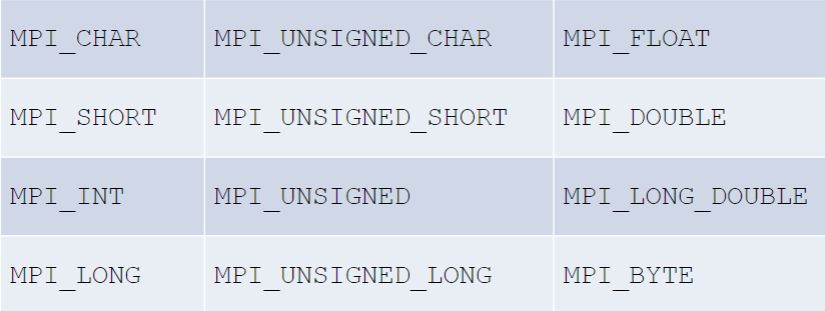
\includegraphics[width=0.7\textwidth]{figures/MPI_datatypes.png}
    \caption{MPI datatypes}
    \label{fig:mpi_datatypes}
\end{figure}


\subsection{Message matching}

Imagine that we have a process \textbf{q} that sends a message, and a process \textbf{r}
that receives it. The message can only be received by \textbf{r} if the following conditions
are met:
\begin{itemize}
    \item The source of the message is \textbf{q}.
    \item The tag of the message is the same as the tag of the receive function. 
    \item The communicator of the message is the same as the communicator of the receive function.
    \item The datatype of the message is the same as the datatype of the receive function.
    \item The count of the message is less than or equal to the count of the receive function.
\end{itemize}

\subsection{Non-overtaking messages}

If a process \textbf{q} sends two messages to a process \textbf{r}, the messages will be
received in the same order they were sent. This is called the \textbf{non-overtaking} property.\\

There is no restriction on the arrival of messages sent from different processes, meaning that
messages sent from different processes can arrive in any order, even if they were sent in a
specific order.

\subsection{Deadlocks in MPI}

A \textbf{deadlock} occur when processes block for communication, but their requests remain
unmatched or otherwise unprocessed. Deadlocks can occur in MPI when two or more processes
are waiting for each other to send or receive messages.\\

For example:

\begin{lstlisting}[language=C++]
if (rank == 0) {
    MPI_Send(&message[0], MAX_STRING, MPI_CHAR, 1, 0, MPI_COMM_WORLD);
    MPI_Recv(&message[0], MAX_STRING, MPI_CHAR, 1, 0, MPI_COMM_WORLD, MPI_STATUS_IGNORE);
}
else if (rank == 1) {
    MPI_Send(&message[0], MAX_STRING, MPI_CHAR, 0, 0, MPI_COMM_WORLD);
    MPI_Recv(&message[0], MAX_STRING, MPI_CHAR, 0, 0, MPI_COMM_WORLD, MPI_STATUS_IGNORE);
}
\end{lstlisting}

There are two processes, 0 and 1. Process 0 sends a message to process 1, and then waits for
a message from process 1. Process 1 sends a message to process 0, and then waits for a message
from process 0. This will cause a deadlock, as both processes are waiting for each other to send a message.\\

There are 2 approaches to avoid this:
\begin{itemize}
    \item Either you smartly rearrange the order of the sends and receives.
    \item Or use non-blocking communication functions (advanced topic).
\end{itemize}

\subsection{Process Hang}

If a process tries to receive a message and there's \textbf{no matching send}, 
the the process will \textbf{block forever}. When you design your MPI programs,
you must ensure that there is a matching send for every receive.\\

Be careful that there are no inadvertent mistakes in calls to \texttt{MPI\_Send} and
\texttt{MPI\_Recv}. If the tags don't match, or if the rank of the destination process is
the same as the rank of the source process, the receive won't match the send. This will
make that, either the program hangs, or the receive is matched with a different send.

\subsection{MPI input and output}

MPI does not specify which processes have acces to which I/O devices. Virtually all
implementations allow all processes in \texttt{MPI\_COMM\_WORLD} to access the standard 
output and standard error streams, but notice that the output from different processes
can be interleaved.\\

To have "sorted" outpur, the common practice is to have the process with rank 0 print
the output, sent by the other processes. This is what we did in the sorted \textbf{Hello, World!}
example.\\

Unlike output, most MPI implementations do not allow all processes to access the standard
input stream. Only the process with rank 0 can access the standard input stream.\\

The common practice is to have the process with rank 0 read the input, and then it broadcasts,
or scatters, the input to the other processes. For this, we need to use the \textbf{collective
communication} functions.

\section{Collective communication}

The collective routines are used to communicate data between all processes in a communicator.
They involve every process in the communicator, are only blocking routines, and transmit only
predefined MPI datatypes. Also, we cannot use tags to identify messages.\\

\textbf{Note:} Be sure that every process in the communicator calls the \textbf{same}
collective function, with the \textbf{same} arguments, to avoid deadlocks.\\

The most common collective communication functions are:
\begin{itemize}
    \item \texttt{MPI\_Bcast}: Broadcasts a message from the process with rank 0 to all other
    processes in the communicator.
    \item \texttt{MPI\_Scatter}: Splits an array into equal-sized chunks and sends each chunk
    to a different process.
    \item \texttt{MPI\_Gather}: Gathers data from all processes in the communicator and stores
    it in an array in the process with rank 0.
    \item \texttt{MPI\_Reduce}: Reduces data from all processes in the communicator to a single
    value in the process with rank 0.
\end{itemize}

\subsection{Broadcast}

The function \texttt{MPI\_Bcast} broadcasts a message from the process with rank 0 to all other
processes in the communicator. It has the following signature:

\begin{lstlisting}[language=C++]
int MPI_Bcast(void* buf, int count, MPI_Datatype datatype, int root, MPI_Comm comm);
\end{lstlisting}

\begin{itemize}
    \item \texttt{buf} is a pointer to the data to be broadcast.
    \item \texttt{count} is the number of elements to be broadcast.
    \item \texttt{datatype} is the type of the elements to be broadcast.
    \item \texttt{root} is the rank of the process that broadcasts the message.
    \item \texttt{comm} is the communicator in which the message will be broadcast.
\end{itemize}

Let us see an example of the \texttt{MPI\_Bcast} function:

\begin{lstlisting}[language=C++]
std::string message;
if (rank == 0) {
    message = "Hello, World!";
}

MPI_Bcast(&message[0], message.size(), MPI_CHAR, 0, MPI_COMM_WORLD);

std::cout << "Process " << rank << " received the message: " << message << std::endl;
\end{lstlisting}

\vspace{1em}

This program will print the following output:

\begin{lstlisting}[language=bash]
$ mpiexec -np 4 ./hello
Process 0 received the message: Hello, World!
Process 1 received the message: Hello, World!
Process 2 received the message: Hello, World!
Process 3 received the message: Hello, World!
\end{lstlisting}

Notice that, when we are on a receiving process (a process with rank $> 0$), we don't need 
to initialize the message variable, as it will be overwritten by the \texttt{MPI\_Bcast} 
function.

\subsection{Reduce}

The function \texttt{MPI\_Reduce} reduces data from all processes in the communicator to a single
value in the process with rank 0. It has the following signature:

\begin{lstlisting}[language=C++]
int MPI_Reduce(const void* sendbuf, void* recvbuf, int count, MPI_Datatype datatype, MPI_Op op, int dest, MPI_Comm comm);
\end{lstlisting}

\begin{itemize}
    \item \texttt{sendbuf} is a pointer to the data to be sent.
    \item \texttt{recvbuf} is a pointer to the memory where the reduced data will be stored.
    \item \texttt{count} is the number of elements to be reduced.
    \item \texttt{datatype} is the type of the elements to be reduced.
    \item \texttt{op} is the operation to be performed.
    \item \texttt{dest} is the rank of the process that will receive the reduced data.
    \item \texttt{comm} is the communicator in which the data will be reduced.
\end{itemize}

This is specially useful when you want to compute the sum of all elements in an array, or the
maximum value of an array, for example. Instead of having the root process compute the result
after receiving all the data, you can use \texttt{MPI\_Reduce} to evenly distribute the work
among all processes.\\

Let us see an example of the \texttt{MPI\_Reduce} function:

\begin{lstlisting}[language=C++]
int number = rank + 1;
int sum;

MPI_Reduce(&number, &sum, 1, MPI_INT, MPI_SUM, 0, MPI_COMM_WORLD);

if (rank == 0) {
    std::cout << "The sum of the numbers is: " << sum << std::endl;
}
\end{lstlisting}

\vspace{1em}

This program will print the following output:

\begin{lstlisting}[language=bash]
$ mpiexec -np 4 ./hello
The sum of the numbers is: 10
\end{lstlisting}

Notice that this program computes the sum of the numbers from 1 to 4, as each process
contributes with its rank + 1. The result is stored in the \texttt{sum} variable of the
process with rank 0. The following diagram explains the distribution of the work:

\begin{figure}[H]
    \centering
    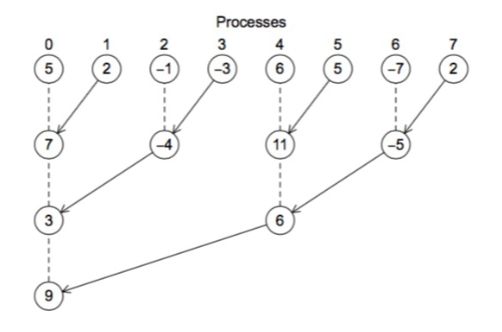
\includegraphics[width=0.6\textwidth]{figures/MPI_reduce.png}
    \caption{MPI reduce for summing numbers}
    \label{fig:mpi_reduce}
\end{figure}

The operations that can be performed with \texttt{MPI\_Reduce} are the following:

\begin{figure}[H]
    \centering
    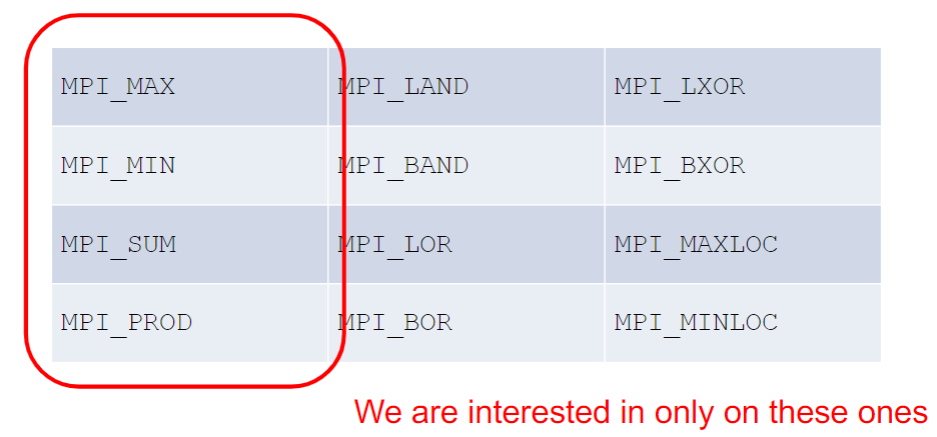
\includegraphics[width=0.7\textwidth]{figures/MPI_operations.png}
    \caption{MPI operations}
    \label{fig:mpi_operations}
\end{figure}

Note that, by using a count argument greater than 1, we can \textbf{reduce arrays} instead of single
values. The following code could thus be used to add a collection of N-dimensional vectors:

\begin{lstlisting}[language=C++]
std::vector<double> local_x (N), sum (N);
// Fill local_x with data (partial computations)
MPI_Reduce(local_x.data(), sum.data(), N, MPI_DOUBLE, MPI_SUM, 0, MPI_COMM_WORLD);
\end{lstlisting}

Also, in some cases we would want for all the processes to receive the result of the reduction.
This can be done by using the \texttt{MPI\_Allreduce} function, which is similar to \texttt{MPI\_Reduce},
but the result is broadcasted to all processes in the communicator. The signature of \texttt{MPI\_Allreduce}
is the same as \texttt{MPI\_Reduce}, but the \texttt{dest} argument is not needed:

\begin{lstlisting}[language=C++]
int MPI_Allreduce(const void* sendbuf, void* recvbuf, int count, MPI_Datatype datatype, MPI_Op op, MPI_Comm comm);
\end{lstlisting}

\subsubsection{Collective comm "IN-PLACE"}

In some cases, you may want to use the same buffer for both the send and receive buffers. This
is called \textbf{in-place} communication.\\

MPI provides the special placeholder \texttt{MPI\_IN\_PLACE} to enable the use of a 
single buffer for both the send and receive buffers. For example:

\begin{lstlisting}[language=C++]
int number = rank + 1;
MPI_Reduce(MPI_IN_PLACE, &number, 1, MPI_INT, MPI_SUM, 0, MPI_COMM_WORLD);
\end{lstlisting}

\subsection{Scatter}

The function \texttt{MPI\_Scatter} splits an array into equal-sized chunks and sends each chunk
to a different process. It has the following signature:

\begin{lstlisting}[language=C++]
int MPI_Scatter(const void* sendbuf, int sendcount, MPI_Datatype sendtype, void* recvbuf, int recvcount, MPI_Datatype recvtype, int root, MPI_Comm comm);
\end{lstlisting}

\begin{itemize}
    \item \texttt{sendbuf} is a pointer to the data to be sent.
    \item \texttt{sendcount} is the number of elements to be sent to each process.
    \item \texttt{sendtype} is the type of the elements to be sent.
    \item \texttt{recvbuf} is a pointer to the memory where the received data will be stored.
    \item \texttt{recvcount} is the number of elements to be received.
    \item \texttt{recvtype} is the type of the elements to be received.
    \item \texttt{root} is the rank of the process that scatters the data.
    \item \texttt{comm} is the communicator in which the data will be scattered.
\end{itemize}

The \texttt{MPI\_Scatter} function implements a form of data distribution called
\textbf{block partition}. The data is divided into blocks of equal size, and each block is
sent to a different process.\\

We can also have a \textbf{cyclic partition}, where the data is divided into blocks of equal
size, but the blocks are sent to the processes in a cyclic order. This implementation is
pretty straightforward, as we can see in the following example:

\begin{lstlisting}[language=C++]
for (size_t i=rank; i < message.size(); i += size) {
    // Do something with message[i]
}
\end{lstlisting}

\begin{figure}[H]
    \centering
    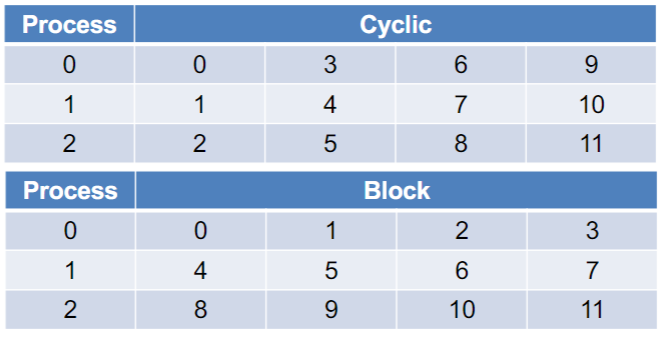
\includegraphics[width=0.7\textwidth]{figures/block_vs_cyclic.png}
    \caption{Block vs cyclic partition}
    \label{fig:block_vs_cyclic}
\end{figure}

For example, we can implement a function that reads a vector of integers from the standard
input, and send block partitions of the vector to different processes:

\begin{lstlisting}[language=C++]
std::vector<int> read_vector(
    unsigned n, std::string const &name, MPI_Comm const &comm
) 
{
    int rank, size;
    MPI_Comm_rank(comm, &rank);
    MPI_Comm_size(comm, &size);
    const unsigned local_n = n / size;
    std::vector<int> result(local_n);

    if (rank == 0) {
        std::vector<int> input(n);
        std::cout << "Enter " << name << "\n";
        for (int &e : input) {
            std::cin >> e;
        }
        MPI_Scatter(input.data(), local_n, MPI_INT, result.data(), 
                    local_n, MPI_INT, 0 comm);
    }
    else {
        MPI_Scatter(nullptr, local_n, MPI_INT, result.data(), 
                    local_n, MPI_INT, 0, comm);
    }
    return result;
}
\end{lstlisting}

We can use this function to implement parallel sum of vectors, for example.

\subsection{Gather}

The \texttt{MPI\_Gather} function joins portions of data from all the processes, storing 
them all in a buffer. It has the following signature:

\begin{lstlisting}[language=C++]
int MPI_Gather(const void* sendbuf, int sendcount, MPI_Datatype sendtype, void* recvbuf, int recvcount, MPI_Datatype recvtype, int root, MPI_Comm comm);
\end{lstlisting}

\begin{itemize}
    \item \texttt{sendbuf} is a pointer to the data to be sent.
    \item \texttt{sendcount} is the number of elements to be sent by each process.
    \item \texttt{sendtype} is the type of the elements to be sent.
    \item \texttt{recvbuf} is a pointer to the memory where the received data will be stored.
    \item \texttt{recvcount} is the number of elements to be received by the root process.
    \item \texttt{recvtype} is the type of the elements to be received.
    \item \texttt{root} is the rank of the process that gathers the data.
    \item \texttt{comm} is the communicator in which the data will be gathered.
\end{itemize}

We can use the \texttt{MPI\_Gather} function to gather and print the results of the parallel
sum of vectors that we implemented with the \texttt{MPI\_Scatter} function:

\begin{lstlisting}[language=C++]
void print_vector(
    vector<int> const &local_v, unsigned n, 
    string const &title, MPI_Comm const &comm
)
{
    int rank, size;
    MPI_Comm_rank(comm, &rank);
    MPI_Comm_size(comm, &size);
    const unsigned local_n = local_v.size();

    if (rank > 0) {
        MPI_Gather(local_v.data(), local_n, MPI_INT, 
                    nullptr, local_n, MPI_INT, 0, comm);
    }
    else {
        vector<int> global_v(n);
        MPI_Gather(local_v.data(), local_n, MPI_INT, 
                    global_v.data(), local_n, MPI_INT, 0, comm);
        cout << title << "\n";
        for (int e : global_v) {
            cout << e << " ";
        }
        cout << endl;
    }
}
\end{lstlisting}

Notice that sometimes, we will need to distribut the gather result on all processes.
This can automatically be done with the \texttt{MPI\_Allgather} function, which is similar
to \texttt{MPI\_Gather}, but the result is broadcasted to all processes in the communicator.
The signature of \texttt{MPI\_Allgather} is the same as \texttt{MPI\_Gather}, but the \texttt{root}
argument is not needed:

\begin{lstlisting}[language=C++]
int MPI_Allgather(const void* sendbuf, int sendcount, MPI_Datatype sendtype, void* recvbuf, int recvcount, MPI_Datatype recvtype, MPI_Comm comm);
\end{lstlisting}

\subsection{Final remarks: collective communication}

We have some final remarks about collective communication:

\begin{itemize}
    \item All the processes in the communicator must call the same collective function.
    For example, if a program attempts to match a call to \texttt{MPI\_Reduce} on one process
    with a call to \texttt{MPI\_Recv} on another process, it is erroneous and probably will
    hang or crash.

    \item The arguments passed by each process to an MPI collective communication must be
    "compatible". For example, if one process passes in 0 as the destination process and 
    another passes in 1, the the outcome of a call to, e.g., \texttt{MPI\_Reduce} is erroneous
    and the program will probably hang or crash.

    \item The \texttt{recvbuf} argument is only used on \texttt{dest} process. 
    However, all of the processes still need to pass in an actual argument corresponding to
    \texttt{recvbuf}, even if it is just \texttt{nullptr}.

    \item Point-to-point communications are matched based on tags and communicators. Collective
    communications don't use tags, so they're mathced solely based on communicator and the 
    order in which they're called.
\end{itemize}




